\documentclass[a4paper, 12pt]{scrreprt}

\pagenumbering{roman}
\setcounter{secnumdepth}{3}
\setcounter{tocdepth}{2} 

\usepackage[german]{babel}
\usepackage[utf8]{inputenc}
\usepackage[T1]{fontenc}
%\usepackage{fancyhdr}
\usepackage{geometry}
\usepackage{lmodern}
\usepackage{verbatim}
\usepackage{graphicx}
\usepackage[hyphens]{url}
\usepackage[pdfborder={0 0 0}]{hyperref}
\usepackage{listings}
\renewcommand\_{\textunderscore\allowbreak}


\usepackage{caption}

\usepackage{amsmath}
\usepackage{blindtext}


\usepackage{fancybox}
\usepackage{makeidx}% \makeindex
\usepackage{lastpage}
\usepackage{natbib}

%\linespread{1.5}
%\geometry{footskip=40pt}
\setcounter{page}{2}
\linespread{1.25}


\begin{document}

\begin{titlepage}
%\includegraphics[scale=0.3]{Z1.png} \hfill
%\includegraphics[scale=0.1]{2.png}\\[1.8cm]
    \begin{center}
    \LARGE \textbf{VirtualDesktop} \\
    \vspace{2.5cm}
    \large\textbf{Projekt}\\
    \vspace{2.5cm}
    \normalsize
    Hochschule RheinMain Wiesbaden \\
    \vspace{2cm}
    \large \textbf{Fortgeschrittene Themengebiete der Informatik\\ Cloud Computing\\}
    \vspace{1cm}
    \normalsize
    Abgabedatum: 30. Januar 2019\\
    \vspace{2.7cm}
    \end{center}
 \normalsize{
    \begin{tabular}{ll}
    	Gruppe: & \\
    	Robin Bergfeld & \\
    	Abiram Pakeerathan & \\
    	Simon Rininsland & \\[0.5cm]
    	Dozent: &\\
        Prof. Dr. Philipp Schaible & \\
    \end{tabular}
    }
\end{titlepage}



\clearpage
\tableofcontents
\clearpage

\pagenumbering{arabic}

%zitieren:
% \cite{Joa10:1}

\chapter{Einführung}
%Mit was, wer wo...
Im Rahmen dieses Projektes ist eine Web-Anwendung unter Verwendung von Amazon Web-Services (AWS) entwickelt worden. Zunächst wird in diesem Kapitel die Idee vorgestellt, anschließend wird die Architektur und die Umsetzung thematisiert.

\section{Projektanforderungen}
%- Welche Anforderungen vom Modul\\
%- Fokus des Projekts
Folgende Projektanforderungen sind umzusetzen:
\\ \\
Es ist eine Web-Anwendung unter Verwendung von Amazon Web-Services (AWS) zu
entwickeln, die mindestens folgende Funktionalitäten beinhalten soll.
\begin{enumerate}
\item Eine statische Web-Seite als Startpunkt der Anwendung.
\item Ausgelagerte REST APIs für dynamisches Verhalten der Anwendung.
\item Benutzerverwaltung mit expliziten Authentifizierungs- und Autorisierungsverwaltung.
\item Die Daten der Anwendung sollen in einer Datenbank verwaltet werden. Die SQL und NoSQL Datenbanken sollen dabei passend eingesetzt werden.
\item Die Anwendung soll mit heterogenen Daten umgehen können. Zusätzlich zu den
organisatorischen Daten (Nutzerverwaltung, Anwendungslogik, etc.) müssen
Multimedia-Daten (Bilder, Audio, Video) integriert werden. Es muss dabei möglich
sein, die Multimedia-Daten entweder herunterzuladen oder zu streamen.
\item Die Anwendung muss horizontal skalierbar sein. (Begründung!)
\end{enumerate}
Zusätzlich haben wir eigene Projektanforderungen hinzugefügt:
\begin{enumerate}
\item Auslegung auf spätere Socketnutzung.
\item Der Code liegt in einen öffentlichen Repo und damit verbunden ...
\item Deploybar von jedermann. Keine statischen Variablen. Der Stack soll mit einen Befehl aufgebaut werden.
\item Strikte Trennung von Model, View und Controller. 
\item Die NodeJS Funktionen sollen möglichst parallel laufen, um wartende Funktionen zu vermeiden.
\item Die EC2 Instanz speichert keine Dateien, sondern \dq schleust\dq\ sie nur durch.
\end{enumerate}

\section{VirtualDesktop}
%- Was mit Bildern (kurz, vielleicht nur ein Bild)\\
%- Funktionen erläutern (MultiWindow, Benutzerverwaltung inkl Rechteverwaltung, Stream, Up-Download, Show)\\
%- Ziel des Produkts (müssen sich mit Anforderungen des Moduls decken)\\

Die Web-Anwendung \textit{VirtualDesktop} soll registrierten Benutzern virtuelle Desktops zur Verfügung stellen, die auf jedem Gerät aufrufbar sind und mit anderen Benutzern geteilt werden können. Die erstellten Desktops sollen zur Multimediaablage genutzt werden. Der Up- und Download ist mit beliebigen Dateitypen möglich. Zusätzlich können Bilder angezeigt sowie Audio- und Video-Daten gestreamt werden.\\[0.25cm]
Alle Benutzer müssen sich anmelden um die Anwendung nutzen zu können. Ein Benutzer kann mehrere Desktops anlegen und diese verwalten. Das Anlegen von mehreren Desktops ist zum Beispiel dann sinnvoll, wenn die Desktops mit unterschiedlichen Personengruppen geteilt werden sollen.
Für jeden angelegten Desktop, kann der Ersteller andere Nutzer hinzufügen und ihnen verschiedene Rechte an seinem Desktop zuweisen.\\
Mit zugewiesenen Leserechten kann der Nutzer Dateien betrachten und herunterladen, mit Schreibrechten darf der Nutzer auch eigene Dateien auf diesem Desktop ablegen. Dem Nutzer müssen explizit Löschrechte zugewiesen werden, um Dateien von fremden Desktops entfernen zu können.\\
Nutzer können auch Admin-Rechte erhalten, sodass diese für den Desktop Nutzerrechte bearbeiten und neue Nutzer hinzufügen dürfen. Ein angelegter Desktop kann aber nur vom Ersteller selbst entfernt werden.\\ 
Es gibt also
\begin{itemize} 
\item[] \textbf{Owner}, die einen oder mehrere Desktops angelegt haben, zwischen diesen wechseln können und andere Nutzer durch Zuweisung von Lese- , Schreib- und Löschrechten zu ihren Desktops hinzufügen dürfen. Sie besitzen für ihre eigenen Desktops alle Rechte. Sie können auch Admin-Rechte, für die Bearbeitung von Nutzerrechten, vergeben.
\item[] \textbf{User}, die Rechte für einen oder mehrere Desktops zugewiesen bekommen haben und zwischen diesen wechseln können und diesen Rechten entsprechend Aktionen ausführen dürfen.
\end{itemize} 

@TODO: Irgendwo muss noch sowas wie "Wie deploye ich" hinein. Also der eine Befehl den man brauch zum erstellen des Stacks.

\begin{figure}[h]
\centering
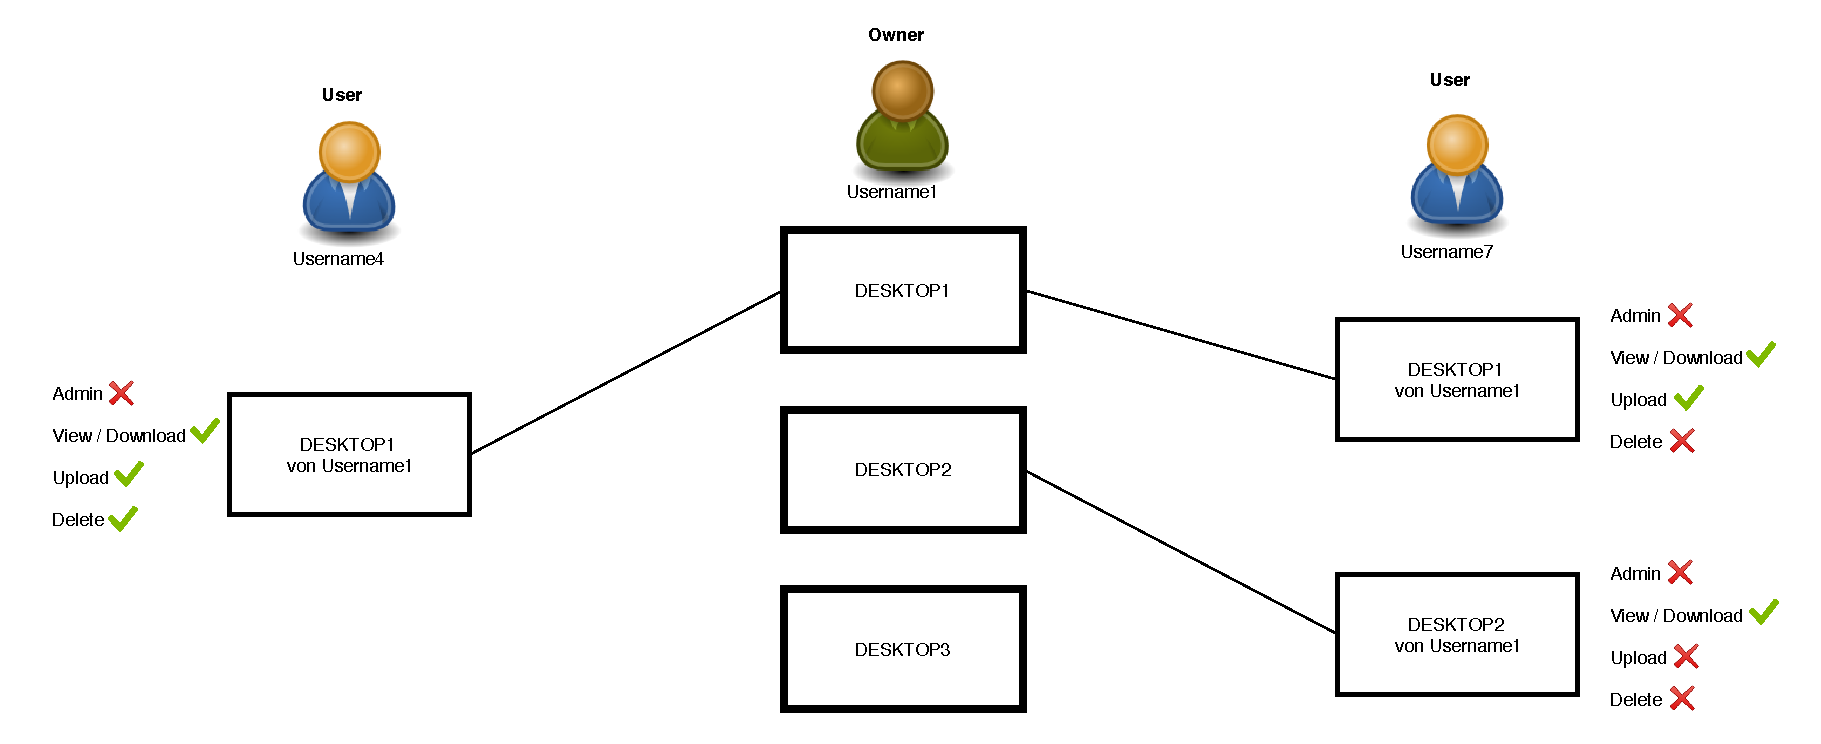
\includegraphics[scale=0.45]{VD_konzept.pdf}
\caption{Username1 ist Owner und besitzt drei Desktops. DESKTOP1 teilt Username1 mit Username4 und Username7. Der DESKTOP2 wird nur mit Username7 geteilt. Den Usern wurden individuell für diese Desktops Rechte zugeteilt. Den DESKTOP3 kann nur der Owner selbst betrachten.}
\end{figure}

\noindent Ein Anwender, der nicht explizit jedem mit dem er seinen Desktop zu teilen vermag, Rechte zuweisen möchte, weil es sich z.B. um eine sehr große Anzahl von Personen handelt, kann als \textit{Owner} seinen Desktop auf public setzen.
Da Desktopnamen in \textit{VirtualDesktop} global eindeutig sind, kann dieser Desktop dann über den Desktopnamen geteilt und gefunden werden.
\textit{User} haben auf einem, auf public gesetzten, Desktop nur Leserechte, außer ihnen wurden explizit weitere Rechte zugewiesen. 
Nur dem \textit{Owner} ist es erlaubt den Desktop wieder auf privat zu setzen, auch \textit{Usern} mit Admin-Rechten für diesen Desktop ist dies nicht gestattet.
 

\chapter{Der Weg in die Cloud}
Es gibt verschiedene Wege, wie man eine Web-Applikation aufsetzt. Die ersten Schritte wird man meist auf eine lokalen Entwicklungsumgebung machen, die man auch zum späteren entwickeln braucht. Irgendwann wird man sich aber die Frage stellen, wo die spätere Infrastruktur laufen wird. \\
Der Weg in die Cloud braucht zu Beginn einen entscheidenden Schritt. Man muss sich für einen Cloudanbieter entscheiden. Es gibt verschiedenste Anbieter wie GoogleCloud von Google, AWS von Amazon oder Azure von Microsoft. \\
Im Rahmen des Moduls CloudComputung an der HS-RM haben wir uns dazu entschlossen die Cloud Services von AWS - Amazon zu nutzen.

\section{Anforderungen an die Cloud}
Unsere Projektanforderungen an die Architektur umfasst einen klassischen Aufbau eines Web Projektes. \\
Das Projekt hat folgende Anforderungen:
\begin{itemize}
\item Eine Laufumgebung auf der NodeJS läuft.
\item Eine Datenbank, die auch mit vielen Zugriffen zurecht kommt. 
\item Einen Speicher, der die Daten von den Nutzern speichert.
\item Alle Zugriffe müssen authentifiziert werden.
\item Skalierung soll möglich sein, um beliebig viele Nutzer bedienen zu können.
\end{itemize}
Es wäre durchaus denkbar fast alle Punkte sehr gut auf einer klassischen, nicht Cloudservice basierende Serverumgebung umzusetzen. Aber spätestens bei der beliebigen Skalierung stößt man auf Probleme. 
\\
Die auf einer klassischen Serverumgebung einfach mögliche vertikale Skalierung stößt schnell auf ihre Grenzen. Früher oder später wird vermutlich die Datenbank in jedem System der Flaschenhals werden und diese dann horizontal zu skalieren ist meist mit großen strukturellen und/oder architektonischen Änderungen verbunden.

\section{Vorteile Infrastruktur}
Eine Umsetzung in AWS bringt ein Umdenken mit sich. In AWS wird jeder Service wird in eigenen Teil gesplittet. Rechner, Speicher, Datenbank, Authentifizierung, Domainverwaltung sogar einzelne Funktionen liegen einzeln in AWS vor. Dadurch ist eine unabhängige Skalierung überhaupt möglich. \\
Um das Projekt umzusetzen brauchen wir uns dank der Cloudservices nicht um dinge, wie den NodsJS Server, den Speicher, die Virtualisierung oder das Netzwerk kümmern. \\
Auch um die Laufzeitumgebung und um das Betriebssystem brauchen wir uns nicht kümmern. Wir legen sie lediglich fest. Dank der Cloudservices von AWS können wir uns nach dem Aufsetzen und Verknüpfen aller unser genutzten Service ganz auf die Programmierung konzentrieren.
\section{Vorteile Skalierung}
Das Hauptproblem von Anwendungen, die erfolgreich von vielen Nutzern genutzt wird ist die Skalierung.
\subsection{Skalierung Plattform / Laufzeitumgebung}
Auf unserer Laufzeitumgebung läuft ein NodeJS Server. Dieser wird durch Elastic-Beanstalk automatisch skaliert. Die Rechenleistung also die CPU, der Arbeitsspeicher wie der interne genutzte Speicher wird dynamisch je nach Bedarf angepasst. \\
Eine klassische Umsetzung auf einen Server kann man lediglich vertikal skalieren und den Arbeitsspeicher oder den CPU aufrüsten. 
\subsection{Skalierung Speicher und Datenbank}
Der Speicher wird bei AWS klassischerweise mit S3 umgesetzt. Der S3 Speicher hat eine Skalierung inkludiert. \\
Es gibt verschiedenste Datenbanktypen, die meisten sind nur schwer skalierbar. AWS bietet die DynamoDB an um Dokumente mit Schlüsselwerten zu speichern. DynamoDB skaliert ebenfalls automatisch. Die globalen DynamoDB Tabellen replizieren sich automatisch über mehrere AWS-Regionen \cite{AWSa}.\\
@TODO: Das Problem mit dem Sachen einzeln holen. nochmal erwähnen. @Robin (ich kann das nicht)
%QUELLE DYNAMODB
%https://aws.amazon.com/de/dynamodb/
\subsection{Skalierung Netzwerk}
Auch um den Datendurchsatz bei der Netzwerkübertragung  braucht man sich dank verteilter Rechenzentren, die sich je nach Nutzungsort verändern können nicht zu kümmern. Plant man einen internationalen Einsatz ist ein Einsatz von Amazon CloudFront / CDN einfach erweiterbar \cite{AWSb}.%QUELLE CLOUDFRONT
%https://aws.amazon.com/de/cloudfront/
\section{Sicherheit}
Sicherheit ist ein großes Thema bei Cloud Services. Anstatt sich händisch darum zu kümmern sein System gegenüber Fremdangriffen zu schützen, kann man bei AWS auf die Expertise von Profis zurückgreifen. Sicherheitspatches werden automatisch eingespielt, über Firewall und Antiviren Programme braucht man sich keine Sorgen mehr machen. \\
Außerdem nimmt AWS mit verschiedenen Services Sicherheitsimplementierungen ab. Cognito ermöglicht schnell und einfach eine Double Opt in Registrierung umzusetzen.
\section{Kosten}
Die Skalierung klassischer Webprojekte läuft so, dass die Infrastruktur für die maximale Nutzung aufgebaut wird. Das bedeutet, dass bei hoher kurzzeitiger Nutzung Ressourcen aufgebaut werden, die dann kurz danach nicht mehr benötigt werden. Ein Rückbau wird selten gemacht und Ressourcen liegen brach.\\
Dieses überpowern der Infrastruktur birgt vermeidbare Mehrkosten. AWS rechnet immer nur den aktuellen Verbrauch ab. Wird ein Server Nachts nicht genutzt, werden keine Kosten generiert. Alle zusätzlichen Kosten einer klassischen Infrastruktur wie Wartung, sind darin bereits inkludiert. 
\chapter{Architektur}
%- Festlegung auf AWS
%- architeturdiagramm
%- Struktur DB und Struktur Anwendungskommunikation- Zusammenhang
HIER DEN AUFBAU ERKLÄREN, DASS IN 3.2 DER ZSMHANG DER SERVICES ERKLÄRT WIRD
- und irgendwo eine tolle Grafik wie die Windows und alles in der DynamoDb und verknüfung mit S3...
Im folgendem wird die Architektur der Webanwendung VirtualDesktop unter Verwendung von Amazon Web Services als Architekturdiagramm dargestellt.
\\
%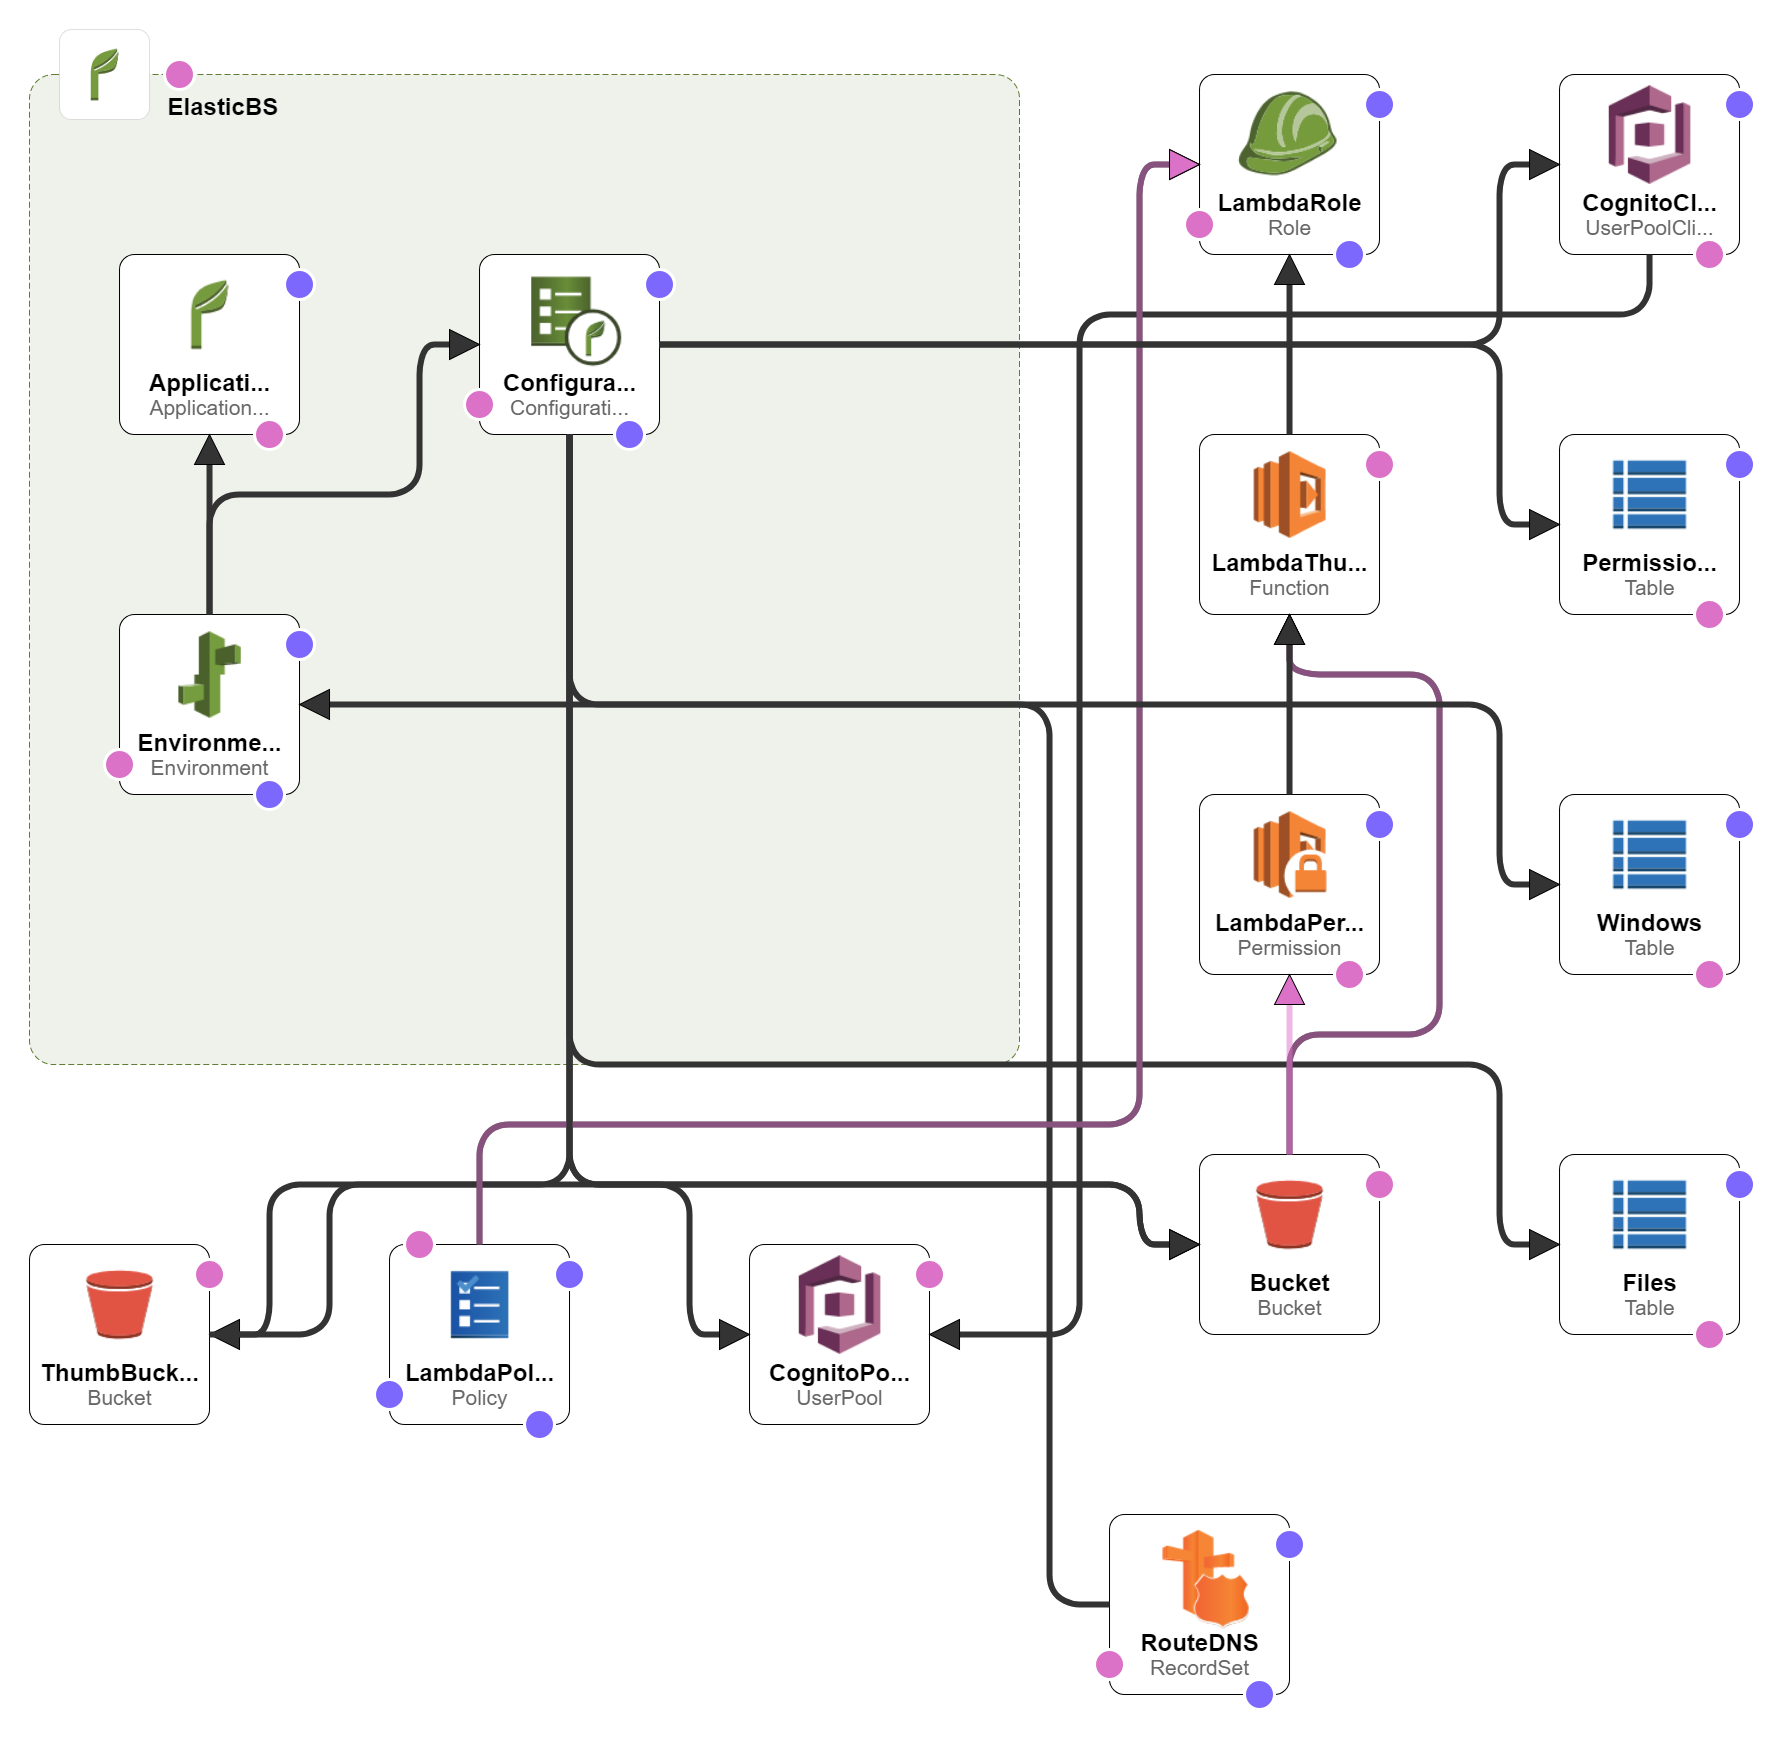
\includegraphics[scale=0.25]{template1-designer.png} 


\section{Elastic Beanstalk Konfiguration}
%-config file
%-  Inkl aller Subservices die EBS anlegt.(LoadBalancer, Security Groups, S3 Bucket für EB Code, Cloudwatch)
%- was es alles mit drin hat aber nebenbei erwähnen immer wieso und
- [WOFÜR IST DIE DATEI GUT? EINLEITEND ERKLÄREN]



\subsection{Authentifizierungsservice Cognito}
Zur Authentifizierung von Nutzern wird der AWS Cognito verwendet. Der Nutzerpool \textit{Cognitopool} vom Typ \textit{AWS::Cognito::UserPool} ist so konfiguriert, dass bei der Registrierung eines neuen Nutzers ein Passwort angegeben werden muss, welches die Minimalvorrausetzung eines AWS-Cognito-Passworts erfüllt (Zeichenlänge von Sechs \cite{AWSD}). Für die Registriereung muss der Nutzer sich verifizieren. Dies geschieht hier über Email, in der der Nutzer seinen Bestätigungscode erhält. Die Formatierung dieser Email wird in \textit{EmailVerificationMessage} und \textit{EmailVerificationSubject} angegeben.  
%COGNITO MINLÄNGE
%https://docs.aws.amazon.com/de_de/AWSCloudFormation/latest/UserGuide/aws-properties-cognito-userpool-passwordpolicy.html
\begin{lstlisting}[xleftmargin=\parindent,numbers=left,numberstyle=\small,numbersep=8pt,frame=L,mathescape=true, basicstyle=\small, language=Java, lineskip={1.0pt}]
CognitoPool:
        Type: AWS::Cognito::UserPool
        Properties:
            AutoVerifiedAttributes:
                -
                    "email"
            EmailVerificationMessage: "Here is your code: {####}"
            EmailVerificationSubject: "Verify your E-Mail for VD"
            Policies:
                PasswordPolicy:
                    MinimumLength: "6"
                    RequireLowercase: false
                    RequireNumbers: false
                    RequireSymbols: false
                    RequireUppercase: false

\end{lstlisting}
\bigskip
\noindent Um den \textit{UserPool} verwenden zu können, benötigt dieser einen Benutzer, den \textit{AWS::Cognito::UserPoolClient}. Dieser wird über die Property \textit{UserPoolId} an den angegeben \textit{UserPool} gebunden, in diesem Fall wird eine Referenz auf den zuvor angelegten UserPool mit dem Namen \textit{CognitoPool} angegeben. Die Property \textit{GenerateSecret} wird hier auf \textit{false} gesetzt, da die clientseitig verwendete Amazon Cognito Identity-SDK für JavaScript keine client secrets unterstützt \cite{AWSAmplify}.
%generateSec QUelle
%https://github.com/aws-amplify/amplify-js/tree/master/packages/amazon-cognito-identity-js

\begin{lstlisting}[xleftmargin=\parindent,numbers=left,numberstyle=\small,numbersep=8pt,frame=L,mathescape=true, basicstyle=\small, language=Java, lineskip={1.0pt}]
    CognitoClient:
        Type: AWS::Cognito::UserPoolClient
        Properties:
            GenerateSecret: false
            UserPoolId: '{"Ref" : "CognitoPool"}'
\end{lstlisting} 

\subsection{Cloud-Speicher S3}
Durch folgende Beschreibung in der Konfiguration wird ein Cloud-Speicher des Typs \textit{AWS::S3::Bucket} angelegt.
\begin{lstlisting}[xleftmargin=\parindent,numbers=left,numberstyle=\small,numbersep=8pt,frame=L,mathescape=true, basicstyle=\small, language=Java, lineskip={1.0pt}]
Bucket:
        Type: AWS::S3::Bucket
\end{lstlisting}          


\subsection{Datenbank DynamoDB}
Das Erstellung einer Datenbanktabelle in der DynamoDB wird hier exemplarisch an der \textit{Permissions}-Tabelle vom Typ \textit{AWS::DynamoDB::Table} gezeigt. Anders als bei klassischen SQL-Datenbanken kann ein Eintrag in einer DynamoDB-Tabelle beliebige Felder beinhalten. Diese werden lediglich über den Schlüssel abgefragt. Um den Schlüssel einer Tabelle zu definieren muss der \textit{AttributeType}, der \textit{AttributeName} und der \textit{KeyType} innerhalb der \textit{AttributeDefinitions} und \textit{KeySchema} angegeben werden. Diese beiden Felder sind erforderlich, müssen also angegeben werden. Das selbe gilt für \textit{ProvisionedThroughput} \cite{AWSDa}.
Dies bedeutet, dass die Skalierung nicht bei der Erstellung durch CloudFormation oder EBS eingestellt werden werden. Um die DynamoDB zu skalieren muss \textit{AWSServiceRoleForApplicationAutoScaling\_DynamoDBTable} im AWS-Account aktiv sein. Falls \textit{AWSServiceRoleForApplicationAutoScaling\_DynamoDBTable} bereits bei der Erstellung durch EB-Deploy aktiviert war skalieren die Tabellen,  ansonsten nicht. Das Autoscaling für die Tabellen kann dann jedoch nachträglich über die Management-Console eingestellt werden. Nähere Informationen hierzu sind in \cite{AWSDb} zu finden.

%QUELLE allg.DYNDB
%https://docs.aws.amazon.com/de_de/AWSCloudFormation/latest/UserGuide/aws-resource-dynamodb-table.html


%QUELLE AUTOSCALING
%https://docs.aws.amazon.com/de_de/amazondynamodb/latest/developerguide/AutoScaling.Console.html


\begin{lstlisting}[xleftmargin=\parindent,numbers=left,numberstyle=\small,numbersep=8pt,frame=L,mathescape=true, basicstyle=\small, language=Java, lineskip={1.0pt}]
Permissions:
        Type: AWS::DynamoDB::Table
        Properties:
            AttributeDefinitions:
                -
                    AttributeName: "Window"
                    AttributeType: "S"
                -
                    AttributeName: "User"
                    AttributeType: "S"
            KeySchema:
                -
                    AttributeName: "Window"
                    KeyType: "HASH"
                -
                    AttributeName: "User"
                    KeyType: "RANGE"
            ProvisionedThroughput:
                ReadCapacityUnits: "1"
                WriteCapacityUnits: "1"
\end{lstlisting}



\subsection{Serverless-Functions Lambda}
Bei der Konfiguration von Lambda in Cloudformation müssen mehrere Ressourcen beachtet werden. \\
Unsere Lambda Funktion benötigt eine Rolle, die sowohl Permissions wie Policies hält. Die Rolle braucht die Erlaubnis Lambda Funktionen aufzurufen, wenn etwas in unseren UserBucket hochgeladen wird. Dies wird folgendermaßen konfiguriert:

\begin{lstlisting}[xleftmargin=\parindent,numbers=left,numberstyle=\small,numbersep=8pt,frame=L,mathescape=true, basicstyle=\small, language=Java, lineskip={1.0pt}]
LambdaPermission:
    Type: "AWS::Lambda::Permission"
    Properties: 
        Action: "lambda:InvokeFunction"
        FunctionName:
            Fn::GetAtt:
            - LambdaThumbnail
            - Arn
        Principal: "s3.amazonaws.com"
\end{lstlisting}

Außerdem wird eine Policy erstellt, um Logs und S3 Objekte zu schreiben und XRAYs verfolgen zu können.\\
Die Lambda Funktion benutzt dann diese Rolle, um alle Dinge zu bewerkstelligen die wir für das erstellen der Thumbnails benötigen. Die Lambda Funktion wird folgendermaßen konfiguriert:

\begin{lstlisting}[xleftmargin=\parindent,numbers=left,numberstyle=\small,numbersep=8pt,frame=L,mathescape=true, basicstyle=\small, language=Java, lineskip={1.0pt}]
LambdaThumbnail:
    Type: "AWS::Lambda::Function"
    Properties: 
        Handler: "index.handler"
        Role: 
            Fn::GetAtt: 
                - "LambdaRole"
                - "Arn"
        Code:
            S3Bucket:
                Ref: CodeBucket
            S3Key: "lambda.zip"
        MemorySize: "1024"
        FunctionName: CreatePhotoThumbnail
        Runtime: "nodejs8.10"
        Timeout: "10"
        TracingConfig:
            Mode: "Active"
\end{lstlisting}

Wie man sieht gibt man in Zeile 3 den Einstiegspunkt mit, benutzt in den folgenden Zeilen die definierte Rolle und greift auf den gezippten Quellcode im definierten CodeBucket zu. Die restlichen Zeilen geben die Parameter für die Laufzeitumgebung an, wie die Arbeitsspeichergröße, den Funktionsname, die Laufzeit, Timeout und das erlaube XRAY Tracing. Auf das XRAY Tracing gehen wir später noch einmal ausführlicher ein.

\subsection{Route53}
Um die generierte ElasticBeanstalk Domain auf eine sprechender Domain zu mappen, in unserem Fall www.virtual-desktop.org, nutzen wir den Route53 Service. Die Konfiguration setzt eine registrierte Route53 Domain bei AWS voraus:

\begin{lstlisting}[xleftmargin=\parindent,numbers=left,numberstyle=\small,numbersep=8pt,frame=L,mathescape=true, basicstyle=\small, language=Java, lineskip={1.0pt}]
RouteDNS:
    Type: AWS::Route53::RecordSet
    Properties:
        HostedZoneName: !Sub
            - ${DName}.
            - DName: !Ref DomainName
        Name: !Sub
            - www.${DName}.
            - DName: !Ref DomainName
        Type: CNAME
        TTL: 900
        ResourceRecords:
        - !GetAtt EnvironmentElasticBS.EndpointURL
\end{lstlisting}

Der Domain Name wird per Startparameter von den Cloudformation Start-Script gesetzt. Per \textit{ResourceRecords} wird die ElasticBeanstalk Domain gesetzt.
 
\section{Zusammenhang der Services}
%- über NodeJS und Express(wegen Datentransformation JSON) ...
%- Auth und Berechtigung prüfen- setzen von Rechten
%- wie sehen die Tabellen aus
%- wie findet das Computing statt
%- kurz jede api-Funktion anreißen
%













\chapter{Besonderheiten}
Einleitung dazu: Weil zu viel gemacht - nur die interessante Teile näher erklärt.

\section{Entwicklungsumgebung lokal / Env- Variablen in NodeJS}
%- Was ist das Problem.\\ 
%- Wie haben wir es gelöst\\
%-  z.B. www Cognito

Bei Elastic-Beanstalk-Projekten wird bei jedem Deploy die gesamte Umgebung mit allen AWS-Resourcen neu gestartet. Dies beinhaltet unter anderem die EC2-Instanz. Da bei Quellcodeänderungen ein Deploy erneut ausgeführt werden muss und die Instanziierung einer EC2-Instanz zeitaufwendig sein kann ist dies für die Entwicklung der Webanwendung nicht praktikabel. Aus diesem Grund wurden in Elastic-Beanstalk, Referenzen \cite{AWSDc} für die dynamisch angelegten Ressourcen erzeugt. Diese Referenzen können in Umgebungsvariablen der EC2-Instanzen übernommen werden, dies geschieht in der \textit{node-env-keys.config} \cite{AWSDd}.\\
Um eine schnellere Entwicklung voranzutreiben wird dieser Umstand genutzt, indem statische (nicht durch EBS-Deploy generiert) Amazon Web Services erstellt und in die Umgebungsvariablen des Entwicklersystems hinzugefügt werden.
Hierbei ist zu beachten, dass lediglich die EC2-Instanzen durch den lokalen Rechner ersetzt werden. Anzulegende Umgebungsvariablen sind
\textit{AWS\_ACCESS\_KEY\_ID} und \textit{AWS\_SECRET\_ACCESS\_KEY} mit den AWS-Credentials, \textit{COGNITO\_CLIENT} und \textit{COGNITO\_POOL} mit der App-Client-ID eines Cognito-Clients (mit GenerateSecret=false) und der Pool-ID des dazugehörigen Cognito-Pools, \textit{FILES}, \textit{PERMISSIONS} und \textit{WINDOWS} mit den jeweiligen Tabellennamen von DynamoDB-Tabellen mit der Struktur beschrieben in [.\textbf{TODO}.] und \textit{BUCKET} sowie \textit{THUMB\_BUCKET} mit den Bucket-Namen. Weiterhin muss die Lambda-Funktion wie in \textbf{LAMDBA TODO} beschrieben  für die Generierung von Thumbnails erstellt werden. Die Lambda-Funktion muss mit den Buckets verknüpft sein.  


%REF QUELLE
%https://docs.aws.amazon.com/de_de/AWSCloudFormation/latest/UserGuide/intrinsic-function-reference-ref.html

%EVI VAR
%https://docs.aws.amazon.com/de_de/elasticbeanstalk/latest/dg/environments-cfg-softwaresettings.html



\section{DynamoDB}
%- Was ist das Problem. Nicht mehrere Sachen löschen nicht möglich.
Da die DynamoDB nicht über die Möglichkeit verfügt, mehrere Einträge über einen Key zu entfernen, muss für die \textit{deleteWindow}-Funktion die gesamte \textit{File}-Liste und \textit{Permission}-Liste für den gegebenen Key eingelesen und jeder Eintrag einzeln in der DynamoDB entfernt werden.
Um nicht jeden Listeneintrag einzeln zu entfernen kann zwar \textit{batchWriteItem} verwendet werden, dieses ist jedoch max. auf 25 DeleteItem-Operationen limitiert und es können keine \textit{conditions} angegeben werden \cite{AWSJSSDKD}. Aus diesem Grund werden die Items, wie hier einleitend erwähnt, einzeln entfernt.

%deleteITEM AWS
%https://docs.aws.amazon.com/AWSJavaScriptSDK/latest/AWS/DynamoDB.html#deleteItem-property

\section{Promise / Dispatcher}
%- Was ist das Problem. Wofür brauchen wir das. Wo war das problem.\\
%- Erklären wieso wieso wir das bauen.\\
%- Erklären was wir gebaut haben und wie.\\
%- kann easy erweitert werden


Die Funktion der AWS-sdk arbeiten mit Callbacks, jedoch sind Aufgaben wie z.B. das Löschen von Desktops und deren Inhalt parallelisierbar, und müssen synchronisiert werden. Um dies zu bewerkstelligen, und um komplexe Callbackstrukturen zu vermeiden wurde eine \textit{dispatch}-Funktion für solche Aufgaben konzipiert. 

\begin{lstlisting}[xleftmargin=\parindent,numbers=left,numberstyle=\small,numbersep=8pt,frame=L,mathescape=true, basicstyle=\small, language=Java, lineskip={1.0pt}]
async function dispatch(tasks, map, callback) {
    var data = { tasks: tasks,
                 map: map, 
                 result: {}, 
                 errors: [], 
                 propergate: true 
    };
    while(data.tasks.length != 0 && data.propergate) {
        var promises = [];
        for (var i = 0; i < tasks[0].length; i++) {
            var f = function(resolve, reject) {
                    this.tasks[0][i](this, () => {
                    resolve();
                });
            };
            promises.push(new Promise(f.bind(data)))
        }
        await Promise.all(promises);
        data.tasks.splice(0, 1);
    }
    callback(data);
}
\end{lstlisting}

Es wird hier zum einen der Parameter \textit{tasks}, einem Array aus Arrays aus Funktionen, der Form \textit{(dis, done)}, sowie ein Objekt \textit{map}, welches innerhalb der \textit{tasks} über \textit{dis.map} zugreifbar ist, und einer \textit{callback}-Funktion, welche nach Beendigung aller \textit{tasks} ausgeführt und die Resultate und Fehler zurückliefert, übergeben. Der \textit{callback} ist notwendig, da die Funktion asynchron ist. Die \textit{dispatch}-Funktion sorgt dafür, dass die Funktionen der inneren \textit{task}-Arrays parallel durch die Kapselung in \textit{promisses} ausgeführt werden. Der Array selbst wird sequentiell ausgeführt, dies wird durch \textit{await} sichergestellt. Es ist zu dem möglich, während des \textit{dispatch}-Prozesses weitere \textit{tasks} hinzuzufügen (dies wird z.B. beim Löschen von Desktops verwendet). Ermöglicht wird dies, da jede \textit{(dis, done)}-Funktion auf das \textit{data}-Objekt und somit auf das Doppelarray aus Funktionen zugreifen kann. Dadurch ist es den Funktionen auch möglich, Ergebnisse in \textit{results} zu speichern, Fehler in \textit{errors} anzugeben und die weitere Ausführung paralleler Arbeitsschritte durch das setzen von \textit{propergate} auf false zu verhindern. Das \textit{dis} der \textit{(dis, done)}-Funktion wird hierbei auf \textit{data} gebinded, das \textit{done} ist hier eine \textit{callback}-Funktion, welche das \textit{resolve} von \textit{Promise} ausführt. Die Funktion \textit{dispatch} kann wie am folgendem Beispiel der \textit{deleteWindow}-Funktion gezeigt verwendet werden:

\begin{lstlisting}[xleftmargin=\parindent,numbers=left,numberstyle=\small,numbersep=8pt,frame=L,mathescape=true, basicstyle=\small, language=Java]

function deleteWindow(username, windowName, callback) {
    var map = { 
        "username": username, 
        "windowName": windowName
    };
    dispatch([[checkParams], 
              [getPermissions], 
              [checkPermissions("owner")], 
              [deleteWindowDynamoDB, 
               removeFilesAndFileInfos, 
               deleteWindowPermissonsDynamoDB
             ]], map, (data) => {
        callback(reply(data));
    });
}
\end{lstlisting}

\noindent Zunächst wird der \textit{username} und \textit{windowName} durch \textit{checkParams} auf Existenz geprüft. Anschließend werden die Berechtigungen für den Benutzer durch \textit{getPermissions} aus der DynamoDB für den angegeben Desktop abgefragt. Die Berechtigungen sind nun im Kontext von \textit{checkPermissions} über \textit{dis.data} zugreifbar. Die \textit{checkPermissions}-Funktion setzt \textit{propagate} auf \textit{false}, falls der Nutzer nicht Besitzer des Desktops ist (und einen Fehler in \textit{dis.errors}-Array schreiben). Ansonsten wird der Desktop und alle dazugehörigen Inhalte und Berechtigungen gelöscht.    

\section{Model-View-Controller}
%- Warum brauchen wir das\\
%- kann easy erweitertert werden\\
%- Wie haben wir es gelöst

Um die parallele Entwicklung des Projektes gewährleisten zu können wird ein Model-View-Controller verwendet. Das Model beinhaltet hierbei die Amazon Web Services S3, DynamoDB, Cognito welche durch die \textit{virtual-desktop.js} in Schnittstellen abstrahiert wird und mittels NodeJS-Express-Server für den Controller zugänglich ist. Diese Abstraktion wurde vorgenommen, damit der NodeJS-Express-Server durch AWS-Lambda substituiert werden kann. Der NodeJS-Express-Server wird durch den Elastic-Beanstalk bereitgestellt. AWS-Lambda wird im Backend verwendet um für neue Dateien, welche durch den Nutzer in den S3-Bucket gespeichert werden Thumbnails zu erstellen.\\
Die Schnittstelle \textit{api.js} im Frontend wird durch den Controller erweitert. Dieser Controller reagiert auf die Eingaben des Nutzers im Frontend, indem Controller-Funktionen angesprochen werden. Bei Bedarf werden Backend-Funktionen durch den Controller angesprochen und/oder im Frontend Events ausgelöst, wodurch dieses aktualisiert werden kann.
Die Verwendung eines Controllers ist vorteilhaft um die spätere Einbindung von Push-Notifications mit geringem Aufwand zu realisieren.



\section{Streaming Download / Upload}
%- Was ist das Problem. Wofür brauchen wir das. Wo war das problem.\\
%- Erklären wieso wieso wir das bauen.\\
%- Erklären was wir gebaut haben und wie.

Um Dateien von und in den S3-Bucket zu laden, können Buffer verwendet werden, dies bedeutet das die Dateien zunächst im Arbeitsspeicher oder im Speicher des NodeJS-Express-Server zwischengespeichert werden müssen. Da eine EC2-Instanz nur über ein begrenztes Volumen an Speicher verfügt, ist das Buffern von Dateien nicht empfehlenswert (erhöhte Kosten, Skalierung von EC2-Instanzen) \cite{AWS}.\\
%https://aws.amazon.com/de/ec2/pricing/on-demand/
Aus diesem Grund werden die Dateien in diesem Projekt vom Backend gestreamt. Hierzu wurden die folgenden Express-Middleware-Bibliotheken geprüft:

\begin{itemize}
\item multer
\item express-fileupload
\item express-busboy
\item busboy-body-parser
\item busboy
\end{itemize}


%TO DO: QUELLEN EINTRAGEN - in .BIB
\noindent Die Middleware \textit{multer} und \textit{express-fileupload} kommen für das gestreamte Hochladen von Dateien auf den S3-Bucket nicht in Frage, da sie keine Streams unterstützen sondern entweder auf der Festplatte speichern  oder im Arbeitsspeicher buffern [quelle: multer, fileupload].
%multer: https://www.npmjs.com/package/multer
%fileupload: https://www.npmjs.com/package/express-fileupload
Um \textit{busboy} im Kontext von NodeJS-Express verwenden zu können, kann \textit{express-busboy} verwendet werden. Allerdings ist diese Bibliothek ebenfalls nur im Stande auf die Festplatte zu speichern. Auch der \textit{busboy-body-parser} stellte sich bei näherer Betrachtung des Quellcode als ungeeignet heraus, da auch dieser nur im Arbeitsspeicher buffert \cite{LeonardMartin}.\\
%https://github.com/lennym/busboy-body-parser/blob/master/index.js
Die Bibliothek \textit{busboy} hingegen liest den HTTP-Request als Stream ein und bietet auch die Dateien als Stream an \cite{busboy}.
%https://www.npmjs.com/package/busboy
Die Problematik, die sich hieraus ergibt, ist das für das Speichern der Datei der Desktop auf dem die Datei gespeichert werden soll bekannt sein muss. Da \textit{busboy} allerdings auf dem HTTP-Request-Stream arbeitet muss der Desktopname vor der Datei im \textit{multipart/form-data} stehen. Um \textit{busboy} zu verwenden wurde daher eine minimalistische Middleware \textit{busboySync.js} entwickelt \cite{Express}.
%https://expressjs.com/en/guide/using-middleware.html
Diese Middleware kommt in allen Resourcen als Router-Middleware des NodeJS-Express-Servers zum Einsatz, welche \textit{multipart/form-data} verarbeitet. Ausnahme hierbei bildet die \textit{/addFile}-Resource, welche aus oben genannten Gründen \textit{busboy} nativ verwendet.\\
Für den Download von Dateien wird die \textit{/getStream}-Resource verwendet, diese liefert für typische Range-Requests der Form
\begin{lstlisting}
bytes=x-y
\end{lstlisting}
, wobei x das Start-byte und y das End-byte darstellt (y kann auch entfallen), ein HTTP-Response-206 (Partial Content) zurück \cite{HTP}.

%QUELLE: Range,206 723
%https://www.rfc-editor.org/rfc/rfc7233.txt 

\section{Lambda - Thumbnailgenerator}
Im Rahmen der Darstellung unseres virtuellen Desktops brauchen wir Thumbnails um eine Vorschau der Bilder auf dem Desktop zu sehen. Für diese Funktion haben wir  uns entschlossen Lambda zu nutzen. Wir nutzen Lambda, um eine einzelne NodeJS-Funktion auszuführen. \\
Die Funktion wird durch ein S3 \textit{s3:ObjectCreated:*} Event gestartet. Das Thumbnail Script filtert zuerst die Bilder aus den Anfragen, anhand der Dateiendungen heraus. Diese Bilder werden daraufhin verkleinert und in einen zweiten Bucket mit denselben Namen hochgeladen. Dieser zweite Bucket hat denselben Namen wie der Ursprungsbucket mit dem Präfix \textit{thumbs}. Damit kann man nun einfach aus dem NodeJS System auf das Thumbnail zugreifen. \\
Ist das Thumbnail nicht vorhanden, wird ein generisches Vorschaubild erzeugt. 
\subsection{XRAY}
Wer eine Lambda Funktion über Cloudformation definiert und hochfährt wird unweigerlich über XRAY stolpern. Mit einer Fehlermeldung wie: 
\begin{lstlisting}
The provided execution role does not have permissions to
call PutTraceSegments on XRAY
\end{lstlisting}
wird die Erstellung abgebrochen. Wird eine Lambda Funktion durch ein Service wie Cloudformation getriggert, braucht Lambda keine weiteren Berechtigungen, da Lambda diese in den Stack-Kontext bereits besitzt. Unser Lambda Service wird aber durch ein Event getriggert. Wenn ein User etwas in den Userbucket lädt, wird die Lambda Funktion ausgeführt. Dadurch fehlt der Funktion der Stack Kontext, auch wenn er durch jenen erstellt wurde. \\
Seit Anfang 2018 \cite{AWSDe} ist es möglich durch hinzufügen von
\begin{lstlisting}
Properties:
  TracingConfig:
    Mode: "Active"
\end{lstlisting} 
in dem Service \textit{AWS::Lambda::Function} und mit 
\begin{lstlisting}
Properties:
  PolicyDocument:
  -
    Effect: Allow
    Action:
    - xray:PutTraceSegments
    - xray:PutTelemetryRecords
    Resource: '*'
\end{lstlisting} 
in dem Lambda Funktion genutzte Policy \textit{AWS::IAM::Policy}
%QUELLE XRAY
%https://docs.aws.amazon.com/de_de/xray/latest/devguide/xray-services-lambda.html




\chapter{Kosten - Aufwände}
Um die etwaigen Kosten abzuschätzen haben wie den \textit{AWS-Gesamtbetriebskostenrechner} bedient. [QUELLE: KOSTENRECHNER] 
%QUELLE KOSTENRECHNER
%https://calculator.s3.amazonaws.com
\section{Entwicklungskosten}
Im Laufe der Umsetzung des Projektes betrachten wir verschiedene Kostenstellen. Als reine Entwicklungskosten bezeichnen wir die Zeit, die wir benötigt haben das reine Produkt zu erstellen ohne die modulspezifischen Anforderungen wie Dokumentation oder die Präsentation. \\
Wir haben im Laufe der Entwicklungszeit mit 3 Personen etwa \textbf{480 Stunden} gebraucht, um das Projekt umzusetzen. Bei einem Stundenlohn von 15 Euro würden sich die Entwicklungskosten auf etwa \textbf{7200 Euro} belaufen. \\
Für die Umsetzung der Präsentation und Dokumentation haben wir etwa \textbf{60 Stunden} verwendet. Bei einem Stundenlohn von 15 Euro würden sich die Entwicklungskosten auf etwa \textbf{900 Euro} belaufen. \\
Würde man solch ein Projekt zur Umsetzung beauftragen, müsste man etwa mit Entwicklungskosten von \textbf{8100 Euro} rechnen.
\section{Einsetzungskosten}
Um die Anwendung unverändert zum laufen zu bringen ist lediglich ein Befehl von Nöten. Dies würde keine Kosten verursachen. \\
Wir haben während der Entwicklung sehr darauf gedachtet die Anwendung möglichst Erweiterbar zu entwickeln. Dies würde Kosten, die bei einer persönlichen Anpassung entstehen würden, gering halten.
\section{Betriebskosten}
- Aufführung der genutzten Services mit Bezug auf Kosten\\
- Hochrechnung pro Monat und pro Nutzer (oder pro 100 Nutzer) \\
- Grafik erstellen

Zur Kalkulation der Betriebskosten betrachten wir die laufenden Monatskosten für die folgenden Szenarien:\\
\begin{itemize}
\item Es werden 10 Anfragen pro Minute gestellt und \textbf{438000} pro Monat.
\item Es werden 1000 Anfragen pro Minute gestellt und \textbf{43800000} pro Monat.
\item Es werden 1000000 Anfragen pro Minute gestellt und \textbf{43800000000} pro Monat.
\end{itemize}

Da die verschiedenen Funktionen unserer Anwendung verschiedene Kosten verursachen gehen wir davon aus, dass die Requests etwa gleich verteilt auf unsere verschiedenen Funktionen aufgegliedert sind wie Einloggen, Desktop wechseln, Bild hochladen, Datei hochladen usw. Dies würde bedeuten, dass die Hälfte der Requests \\
Für die Berechnung wurde der AWS Simply Monthly Calculator Rechner bedient. [QUELLE: AWSRECHNER] Für Lambda wurde folgender Rechner genutzt. [QUELLE: LAMBDARECHNER]
\\
Wir setzen folgende Variablen fest:
\begin{lstlisting}
MINUTE-REQUESTS: Minuetliche Requests
MONTH-REQUESTS: Totale monatliche Requests
\end{lstlisting} 
Damit würden sich dann folgende Parameter ergeben, die jeweils für die verschiedenen Szenarien in den \textit{AWS Simply Monthly Calculator} einzutragen sind.
\begin{enumerate}
\item EC2 Instanz
\begin{enumerate}
\item Amazon EC2-Instances: 1/10 * MINUTE-REQUESTS
\item Typ: Linux für m1.small
\item EBS-Volumes: 1/10 * MINUTE-REQUESTS
\item EBS-Volumes-Speicher: 2GB Speicher
\item Ausgehende Datenübertragungen: 1/10 MINUTE-REQUESTS TB pro Monat
\item Eingehende Datenübertragungen: 1/10 MINUTE-REQUESTS TB pro Monat
\end{enumerate}
\item S3 Requests
\begin{enumerate}
\item Standard Storage: 10 * \textit{MINUTE-REQUESTS} in GB
\item PUT/COPY/POST/LIST Requests: 1/3 * \textit{MONTH-REQUESTS}
\item GET- und andere Anfragen: 2/3 * \textit{MONTH-REQUESTS}
\item Data Returned by S3 Select: 10 * \textit{MINUTE-REQUESTS}
\end{enumerate}
\item Lambda Requests
\begin{enumerate}
\item Executian a Month: 1/5 * MONTH-REQUESTS
\item Memory Allocation in MB: 256
\item Duration in MS: 2000
\end{enumerate}
\item DynamoDB
\begin{enumerate}
\item Größe Datenvolumen: 1 GB
\item Elementgröße: 1 KB
\item Total number of items read per second: 1/60 * MINUTE-REQUESTS
\item Number of items written per second: 1/60 * MINUTE-REQUESTS
\end{enumerate}
\item Route53
\begin{enumerate}
\item Hostet Zones: 1
\item Standardabfragen: MONTH-REQUESTS
\end{enumerate}
\end{enumerate}

\begin{figure}[h]
\centering
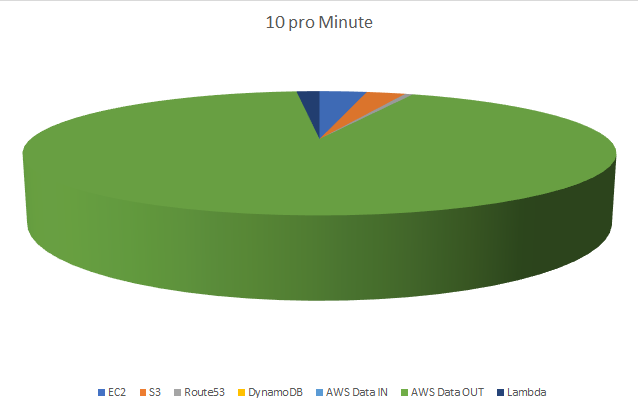
\includegraphics[scale=1]{costs-10.png}
\caption{Kosten für 10 Requests pro Minute}
\end{figure}
\begin{figure}[h]
\centering
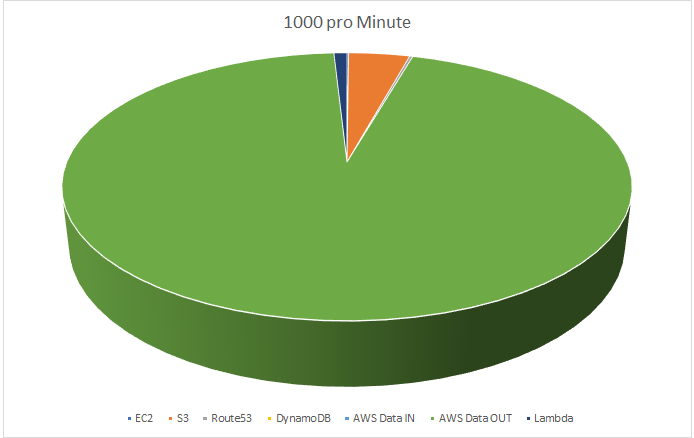
\includegraphics[scale=1]{costs-1000.png}
\caption{Kosten für 1000 Requests pro Minute}
\end{figure}
\begin{figure}[h]
\centering
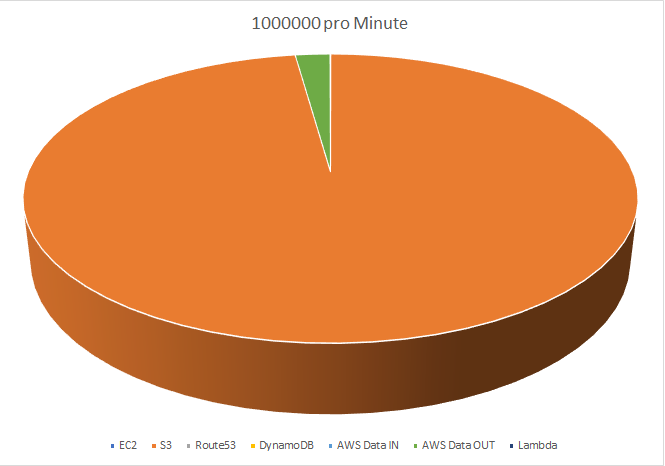
\includegraphics[scale=1]{costs-1000000.png}
\caption{Kosten für 1000000 Requests pro Minute}
\end{figure}

asd

%10 = https://calculator.s3.amazonaws.com/index.html?lng=de_DE#key=calc-D24F7D67-4399-487A-90EE-BFB707E5B259&r=FRA
%1000 = https://calculator.s3.amazonaws.com/index.html?lng=de_DE#key=calc-A2F36303-B150-4A4B-8BAD-3E8EAB946274&r=FRA
%1000000 = https://calculator.s3.amazonaws.com/index.html?lng=de_DE#key=calc-77814ED1-00F9-4058-8401-E0D1D464D215&r=FRA


%QUELLE LAMBDARECHNER
%https://dashbird.io/lambda-cost-calculator/
%QUELLE AWSRECHNER
%https://calculator.s3.amazonaws.com

\clearpage
\bibliographystyle{alpha}
\bibliography{documentation}
%\bibliographystyle{apalike}

\end{document}